Im folgenden Kapitel sollen zunächst einige wissenschaftlichen Arbeiten zu dem untersuchten Thema vorgestellt und zu dieser Arbeit abgegrenzt werden.

\begin{figure}[ht]
  \centering
  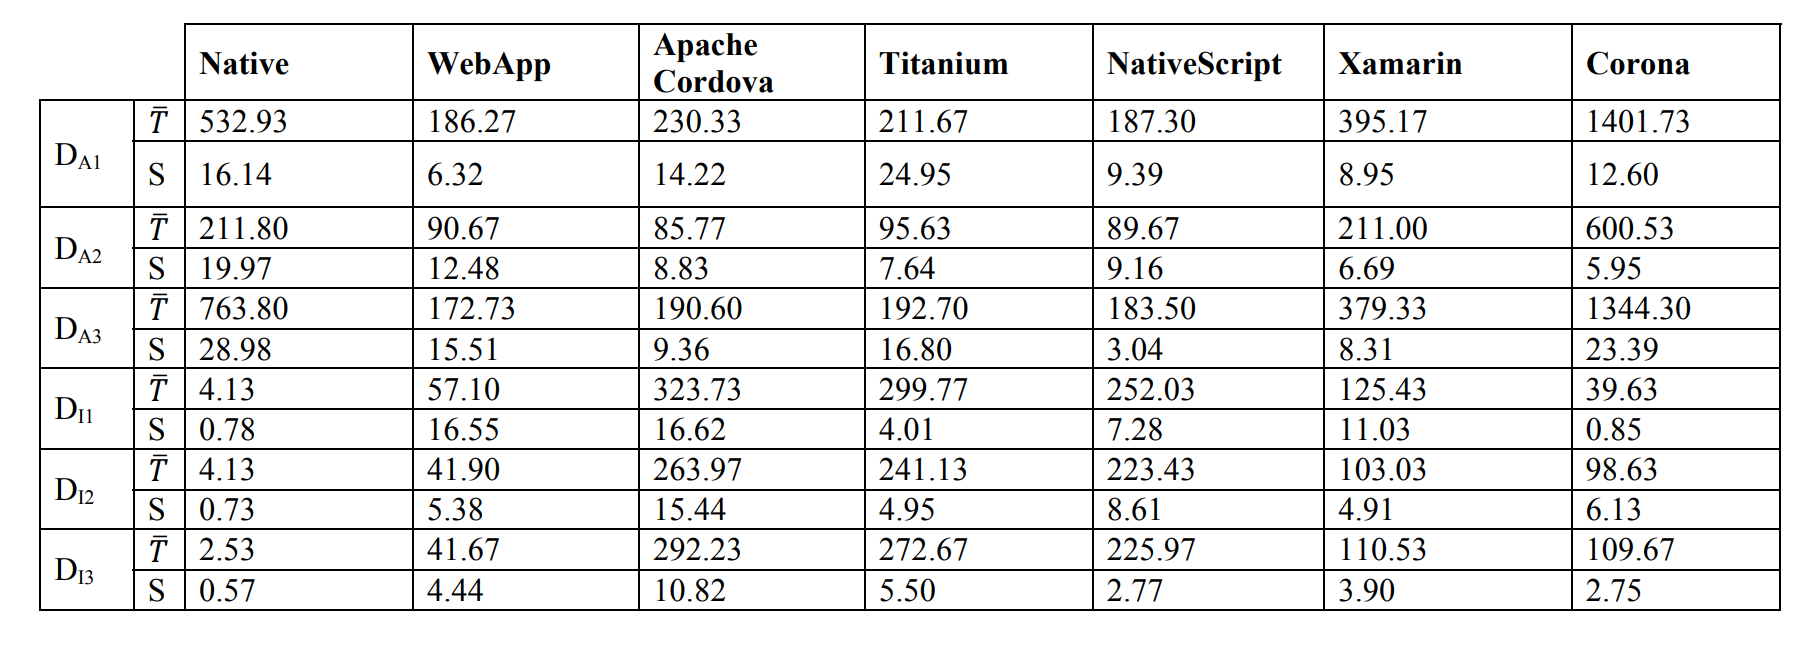
\includegraphics[width=\textwidth,keepaspectratio]{images/IEEE_Delia_Al.png}
  \caption[Ergebnistabelle der Performancemessungen von Delia et al]{Ergebnistabelle der Performancemessungen von Delia et al \cite{IEEE_development_classes}}
  \label{fig:result_table_IEEE_related_work}
\end{figure}

Einige Arbeiten untersuchen den Faktor Performance. Delia et al \cite{IEEE_development_classes} etwa testen die Performance anhand von komplexen Berechnungen und zeichnen dabei die verstrichene Zeit für iOS und Android auf. Sie berechnen außerdem die Standardabweichung, um zu untersuchen, wie gleichmäßig die Ergebnisse sind. In Abbildung \ref{fig:result_table_IEEE_related_work} kann die Ergebnistabelle betrachtet werden. D$_x$ definiert das Testgerät, wobei x das Betriebssystem spezifiziert. $\overline T$ ist die Zeit in Millisekunden, die die Berechnung benötigt hat und S die Standardabweichung. Dabei ist ein möglichst kleiner Wert von $\overline T$ und S optimal. Sie stellen einen Performance Unterschied zwischen Android und iOS fest, führen diesen jedoch auf die unterschiedliche Hardware der Testgeräte zurück. Insgesamt ermitteln sie eine gute Performance von Web-Applikationen im Vergleich zu den anderen untersuchten Applikationen. Die native Applikation schnitt auf Android schlechter ab als ein Großteil der restlichen untersuchten Ansätze, auf iOS jedoch war dieser Ansatz der schnellste.

In dieser Arbeit werden alle Tests auf einem Gerät durchgeführt, um Vergleichbarkeit zu erlangen. Außerdem wird die Arbeit lediglich auf Android beschränkt, um auf die unterschiedlichen Ansätze und nicht auf die Unterschiede zwischen den Plattformen einzugehen.
 
Denko et al \cite{Denko_performance} vergleichen neben der verbrauchten Zeit für Berechnungen ebenfalls die Auslastung der Geräte während den verschiedenen Aufgaben sowie die App-Größe der kompilierten Apps. Dabei konnten sie feststellen, dass je nach Aspekt, unterschiedliche Ansätze einen besseren Wert aufwiesen. So war etwa bei der Ausführung eines Sortier-Algorithmus die Native Implementierung die schnellste, jedoch hatte der Cross-Kompilierte Ansatz die geringste Auslastung der CPU. Sie kommen daher zum Schluss, dass kein Ansatz in der Performance der Beste ist und deswegen andere Faktoren betrachtet werden müssen, um eine fundierte Entscheidung zu treffen.

Einige Arbeiten vergleichen lediglich die Unterschiede zwischen zwei Ansätzen. So auch Andersson \cite{Andersson_2022}, der in seiner Arbeit die Performance-Unterschiede zwischen einer nativ und einer mit Flutter geschriebenen Cross-Plattform Android App vergleicht. Dabei untersuchte er verschiedene Funktionalitäten, die in vielen Apps vorkommen. Zum Beispiel nachladende Listen oder auch Datenbankoperationen. Das Ergebnis seiner Arbeit ist, dass kein eindeutig besserer Ansatz identifiziert werden kann, da Flutter schneller und ressourcenschonender bei der Dekodierung von Dateien ist, während Animationen auf der nativen Anwendung besser laufen. Er stellt dabei fest, dass der Cross-Plattform-Ansatz insgesamt keine schlechtere Performance als die native Entwicklung aufzeigt.

Die Arbeiten von Andersson \cite{Andersson_2022} und Denko et al \cite{Denko_performance} identifizierten die Performance als keinen eindeutigen Faktor um eine Wahl treffen zu können. Deswegen werden in dieser Arbeit weitere Faktoren in den Vergleich einbezogen.

\begin{table}[ht]
    \centering
    \caption[Ergebnistabelle der Untersuchung von Biørn-Hansen et al]{Ergebnistabelle der Untersuchung von Biørn-Hansen et al \cite{BirnHansen.2020}}
    \begin{tabularx}{13.27cm} { 
  | >{\raggedright\arraybackslash}r 
  || >{\raggedleft\arraybackslash}r 
  | >{\raggedleft\arraybackslash}r 
  | >{\raggedleft\arraybackslash}r
  | >{\raggedleft\arraybackslash}r 
  | >{\raggedleft\arraybackslash}r 
  | >{\raggedleft\arraybackslash}r | }
        \hline
        Framework & TTC & CPU & PreRAM & RAM & ComputedRAM & $\sum_{}{}$\\
        \hline
        Native & 5 & 4 & 6 & 6 & 3 & 24\\
        \hline
        MAML/MD$_2$  & 4 & 5 & 5 & 5 & 4 & 23\\
        \hline
        NativeScript & 6 & 6 & 3 & 3 & 2 & 20\\
        \hline
        React Native & 2 & 1 & 4 & 4 & 5 & 16\\
        \hline
        Flutter & 3 & 3 & 1 & 2 & 6 & 15\\
        \hline
        Ionic & 1 & 2 & 2 & 1 & 1 & 7\\
        \hline
    \end{tabularx}
    \label{fig:result_table_Biorn}
\end{table}

Biørn-Hansen et al \cite{BirnHansen.2020} konzentrierten sich bei ihrer Untersuchung vor allem auf die Nutzung plattformspezifischer Schnittstellen, wie etwa der Geo-Daten oder Kontakte-API. Sie untersuchten dabei neben der verstrichen Zeit, die CPU-Auslastung, die minimale (PreRAM) und maximale RAM Auslastung sowie den für die Aufgabe benötigten RAM (ComputedRAM). Bei der Auswertung dieser fünf Kriterien gewichten sie jeden, der sechs implementierten Ansätze, anhand einer Zahl von eins bis sechs. Die höchste Zahl wird der Implementierung zugeordnet, die am besten in diesem Bereich abgeschlossen hat und eins, die die schlechtesten Ergebnisse lieferte. Danach werden die erreichten Punkte zusammengerechnet. Wie in Tabelle \ref{fig:result_table_Biorn} zu sehen ist, kam der native Ansatz dabei auf den ersten Platz mit einer Punktzahl von 24 Punkten. Das Cross-Plattform-Framework Flutter hingegen landete auf dem vorletzten Platz mit gerade einmal 15 Punkten. In ihrem Fazit halten sie dementsprechend fest, dass die Nutzung von anderen Technologien zu einer Performance-Verschlechterung führen kann, jedoch einige Frameworks in gewissen Bereichen besser abschneiden als die native Implementierung und es somit auf die genauen Anforderungen ankommt.

In ihrer Arbeit bewerten Biørn-Hansen et al \cite{BirnHansen.2020} die verschiedenen Ansätze anhand der gemessenen Werte. Dies führt dabei jedoch zu einer Verzerrung der Ergebnisse, da in einigen Kategorien die Unterschiede nur sehr gering waren, dies aber durch die Art ihrer Bewertung nicht berücksichtigt wird. Deswegen soll in der Arbeit von einer Gewichtung abgesehen werden und anhand von Kriterien Empfehlungen zu gewissen Technologien aufgeführt werden.

Raj und Tolety \cite{IEEE_Rahul_Seshu} stellen in ihrer Arbeit eine Einteilung von Applikationen in vier unterschiedliche Kategorien vor. Diese sind Applikationen,
\begin{itemize}
    \item die hauptsächlich eine Anzeige von Server Daten sind,
    \item die durch Nutzereingaben oder Sensoren Daten erhalten und diese verarbeiten,
    \item die ein eigenständiges System sind und keinerlei Verbindung zu einem Server benötigen,
    \item die einen hohen Kommunikationsgrad mit einem Server haben.
\end{itemize}
Sie empfehlen, dass Entwickler den Entwicklungsansatz anhand der App-Kategorie wählen. Beispielsweise empfehlen sie, dass bei viel Kommunikation mit einem Server der Web-gestützte Ansatz gewählt wird. Sie sagen jedoch auch, dass Cross-Plattform-Lösungen gut sind, wenn mehrere Plattformen abgedeckt werden sollen, da dadurch Entwicklungszeit und Kosten gespart werden können.

Ihre Erklärungen sind nachvollziehbar, jedoch fehlen in ihrer Arbeit Zahlen oder Entscheidungsfaktoren, um ihre Empfehlung zu stützen. Dazu wird in ihrer Auswertung die Klasse der nativen Applikationen vernachlässigt. In dieser Arbeit soll deshalb anhand von konkreten Zahlen und Quellen ein Vergleich zwischen den implementierten Ansätzen gezogen werden, um eine nachvollziehbare Entscheidung zu stützen.

Olsson \cite{Olsson_2020} untersucht in ihrer Arbeit neben der Performance vor allem die Benutzeroberfläche. Dafür implementiert sie native Applikationen für iOS und Android und eine Cross-Plattform Flutter App, die auf beiden Plattformen installiert werden kann. Ihre Performancemessung zeigt, dass die Cross-Plattform-Applikation eine etwas schlechtere Performance als die nativen Implementierungen aufweist. Im zweiten Teil der Untersuchung befragt sie eine Gruppe an Entwicklern und zeigt ihnen unterschiedliche Anwendungsfälle der Android Implementierungen. Danach fragt sie nach Unterschieden und Auffälligkeiten zwischen den zwei anonymisierten Applikationen. Das Ergebnis ist, dass die Mehrheit der Befragten keinen Unterschied zwischen den zwei Anwendungen finden konnten. Der dritte Faktor ihrer Arbeit ist die Programmlänge. Dabei hat die Flutter Implementierung die geringste Anzahl an Zeilen. Am Ende stellt sie fest, dass Flutter eine gute Alternative zur nativen Entwicklung sein kann, dies jedoch abhängig sei von der weiteren Entwicklung des Frameworks.
\newline

Die Arbeit von Olsson \cite{Olsson_2020} stellt eine umfangreiche Untersuchung zwischen den beiden betrachteten Ansätzen dar. Jedoch ist die Arbeit nur auf zwei Ansätze beschränkt und bietet so lediglich einen Vergleich zwischen den Beiden. Um mehr Aussagekraft über verschiedene Ansätze zu erhalten, sollen deswegen in dieser Arbeiten mehr Ansätze untersucht werden. 

Khachouch et al \cite{IEEE_Khackouch_Al} erstellen in ihrer 2020 vorgestellten Arbeit einen Entscheidungsgraphen. Durch die Beantwortung einiger Fragen, sollen Entwickler neuer Applikationen die für ihr Projekt passende Entwicklungsmethodik finden. Als Erstes suchten sie dafür passende Fragen, die eine Eingrenzung erlauben und ordnen diesen ein Gewicht zu, um die Höhe der Frage in dem Graph festzulegen. Sie stellen am Ende fest, dass wenn es keine Einschränkungen in den Bereichen Entwicklungszeit und Kosten gibt, der native Ansatz aufgrund der besseren Performance und Qualität die beste Lösung bleibt. Durch ihren Graphen wird jedoch auch klar, dass oft andere Ansätze sinnvoller sein können.

Der von Kachouch et al \cite{IEEE_Khackouch_Al} vorgestellte Graph liefert innerhalb von zwei bis acht Fragen eine eindeutige Antwort. In dieser Arbeit hingegen soll lediglich eine Tendenz aufgezeigt werden, da jedes Projekt durch seine einzelnen Funktionalitäten sehr komplex ist und nicht mit wenigen Fragen exakt eingeordnet werden kann. Stattdessen soll ein besseres Verständnis vermittelt werden, welche Faktoren eine Entscheidung beeinflussen können. 